\documentclass[10pt,twocolumn,letterpaper]{article}

\usepackage{cvpr}
\usepackage{xfrac}
\usepackage{times}
\usepackage{epsfig}
\usepackage{graphicx}
\usepackage{listings}
\usepackage{amsmath}
\usepackage{amssymb}
\usepackage{color, soul}
\usepackage{float}
\usepackage[super]{nth}
\setlength{\intextsep}{5pt}
\usepackage[nodisplayskipstretch]{setspace}
\setstretch{1}
\usepackage{algorithm}
\usepackage{algorithmic}
\usepackage[utf8]{inputenc}

% Include other packages here, before hyperref.

% If you comment hyperref and then uncomment it, you should delete
% egpaper.aux before re-running latex.  (Or just hit 'q' on the first latex
% run, let it finish, and you should be clear).
\usepackage[breaklinks=true,bookmarks=false]{hyperref}

\cvprfinalcopy % *** Uncomment this line for the final submission

\def\cvprPaperID{****} % *** Enter the CVPR Paper ID here
\def\httilde{\mbox{\tt\raisebox{-.5ex}{\symbol{126}}}}

% Pages are numbered in submission mode, and unnumbered in camera-ready
%\ifcvprfinal\pagestyle{empty}\fi
\setcounter{page}{1}
\begin{document}

%%%%%%%%% TITLE
\title{Pattern Recognition Coursework 2}

\author{Jakub Mateusz Szypicyn\\
CID: 00846006\\
EEE4\\
{\tt\small jms13@ic.ac.uk}
% For a paper whose authors are all at the same institution,
% omit the following lines up until the closing ``}''.
% Additional authors and addresses can be added with ``\and'',
% just like the second author.
% To save space, use either the email address or home page, not both
\and
Jacobus Jukka Hertzog\\
CID: 00828711\\
EEE4\\
{\tt\small jjh13@ic.ac.uk}
}

\maketitle
%\thispagestyle{empty}

%%%%%%%%% ABSTRACT
\begin{abstract}
Line 1\\

Line 2\\

Line 3\\
\end{abstract}

\section{Introduction}
Line 1\\

Line 2\\

Line 3\\
\section{Distance Metrics}
\subsection{Distribution of Wine Data}

The wine data ({\tt\small wine.csv}) provided consisted of three classes. It cis made up of 13 features representing chemical and optical information. The data can be analysed \textit{talis qualis}, however a more elaborate method is to investigate the covariance matrices. The raw data can supply us with information such as feature distribution (mean or spread), whereas covariance matrices will provide the dependency between features. This can be performed for all data altogether or for each class individually. Both methods will result in meaningful information as described in sections \ref{sec:CovAll} and \ref{sec:CovCla}. Furthermore the data was then normalised and the above was repeated.\footnote{Note that data was first separated as per instruction. Only training data is now being considered.} 

\vspace{-3mm}

\subsubsection{All Classes} \label{sec:CovAll}

\indent \indent By investigating the data from all classes we will see that data varies altogether. We can investigate each feature and see what part of space it occupies. We can also determine how strongly all features are related to one another for all classes. Let us begin by examining the distributions of the raw data. The means of the feature distributions vary from around 0.36 for nonflavanoid phenols, through values of 1 to 3 and 10 to 100 to a single extreme at 737.1 for proline. The corresponding deviations are also quite spread out. The general trend is that the larger the mean the larger the standard deviation of the distribution. For example proline distribution has a standard deviation of 287 over 118 samples. The distributions of the features don't always seem to follow bell-shaped Gaussian distribution. However it should be noted that each distribution is in fact a sum of three independent distributions. Distribution of proline in Figure \ref{fig:DistProline} resembles a gamma distribution.

\begin{figure}[H]
\centering
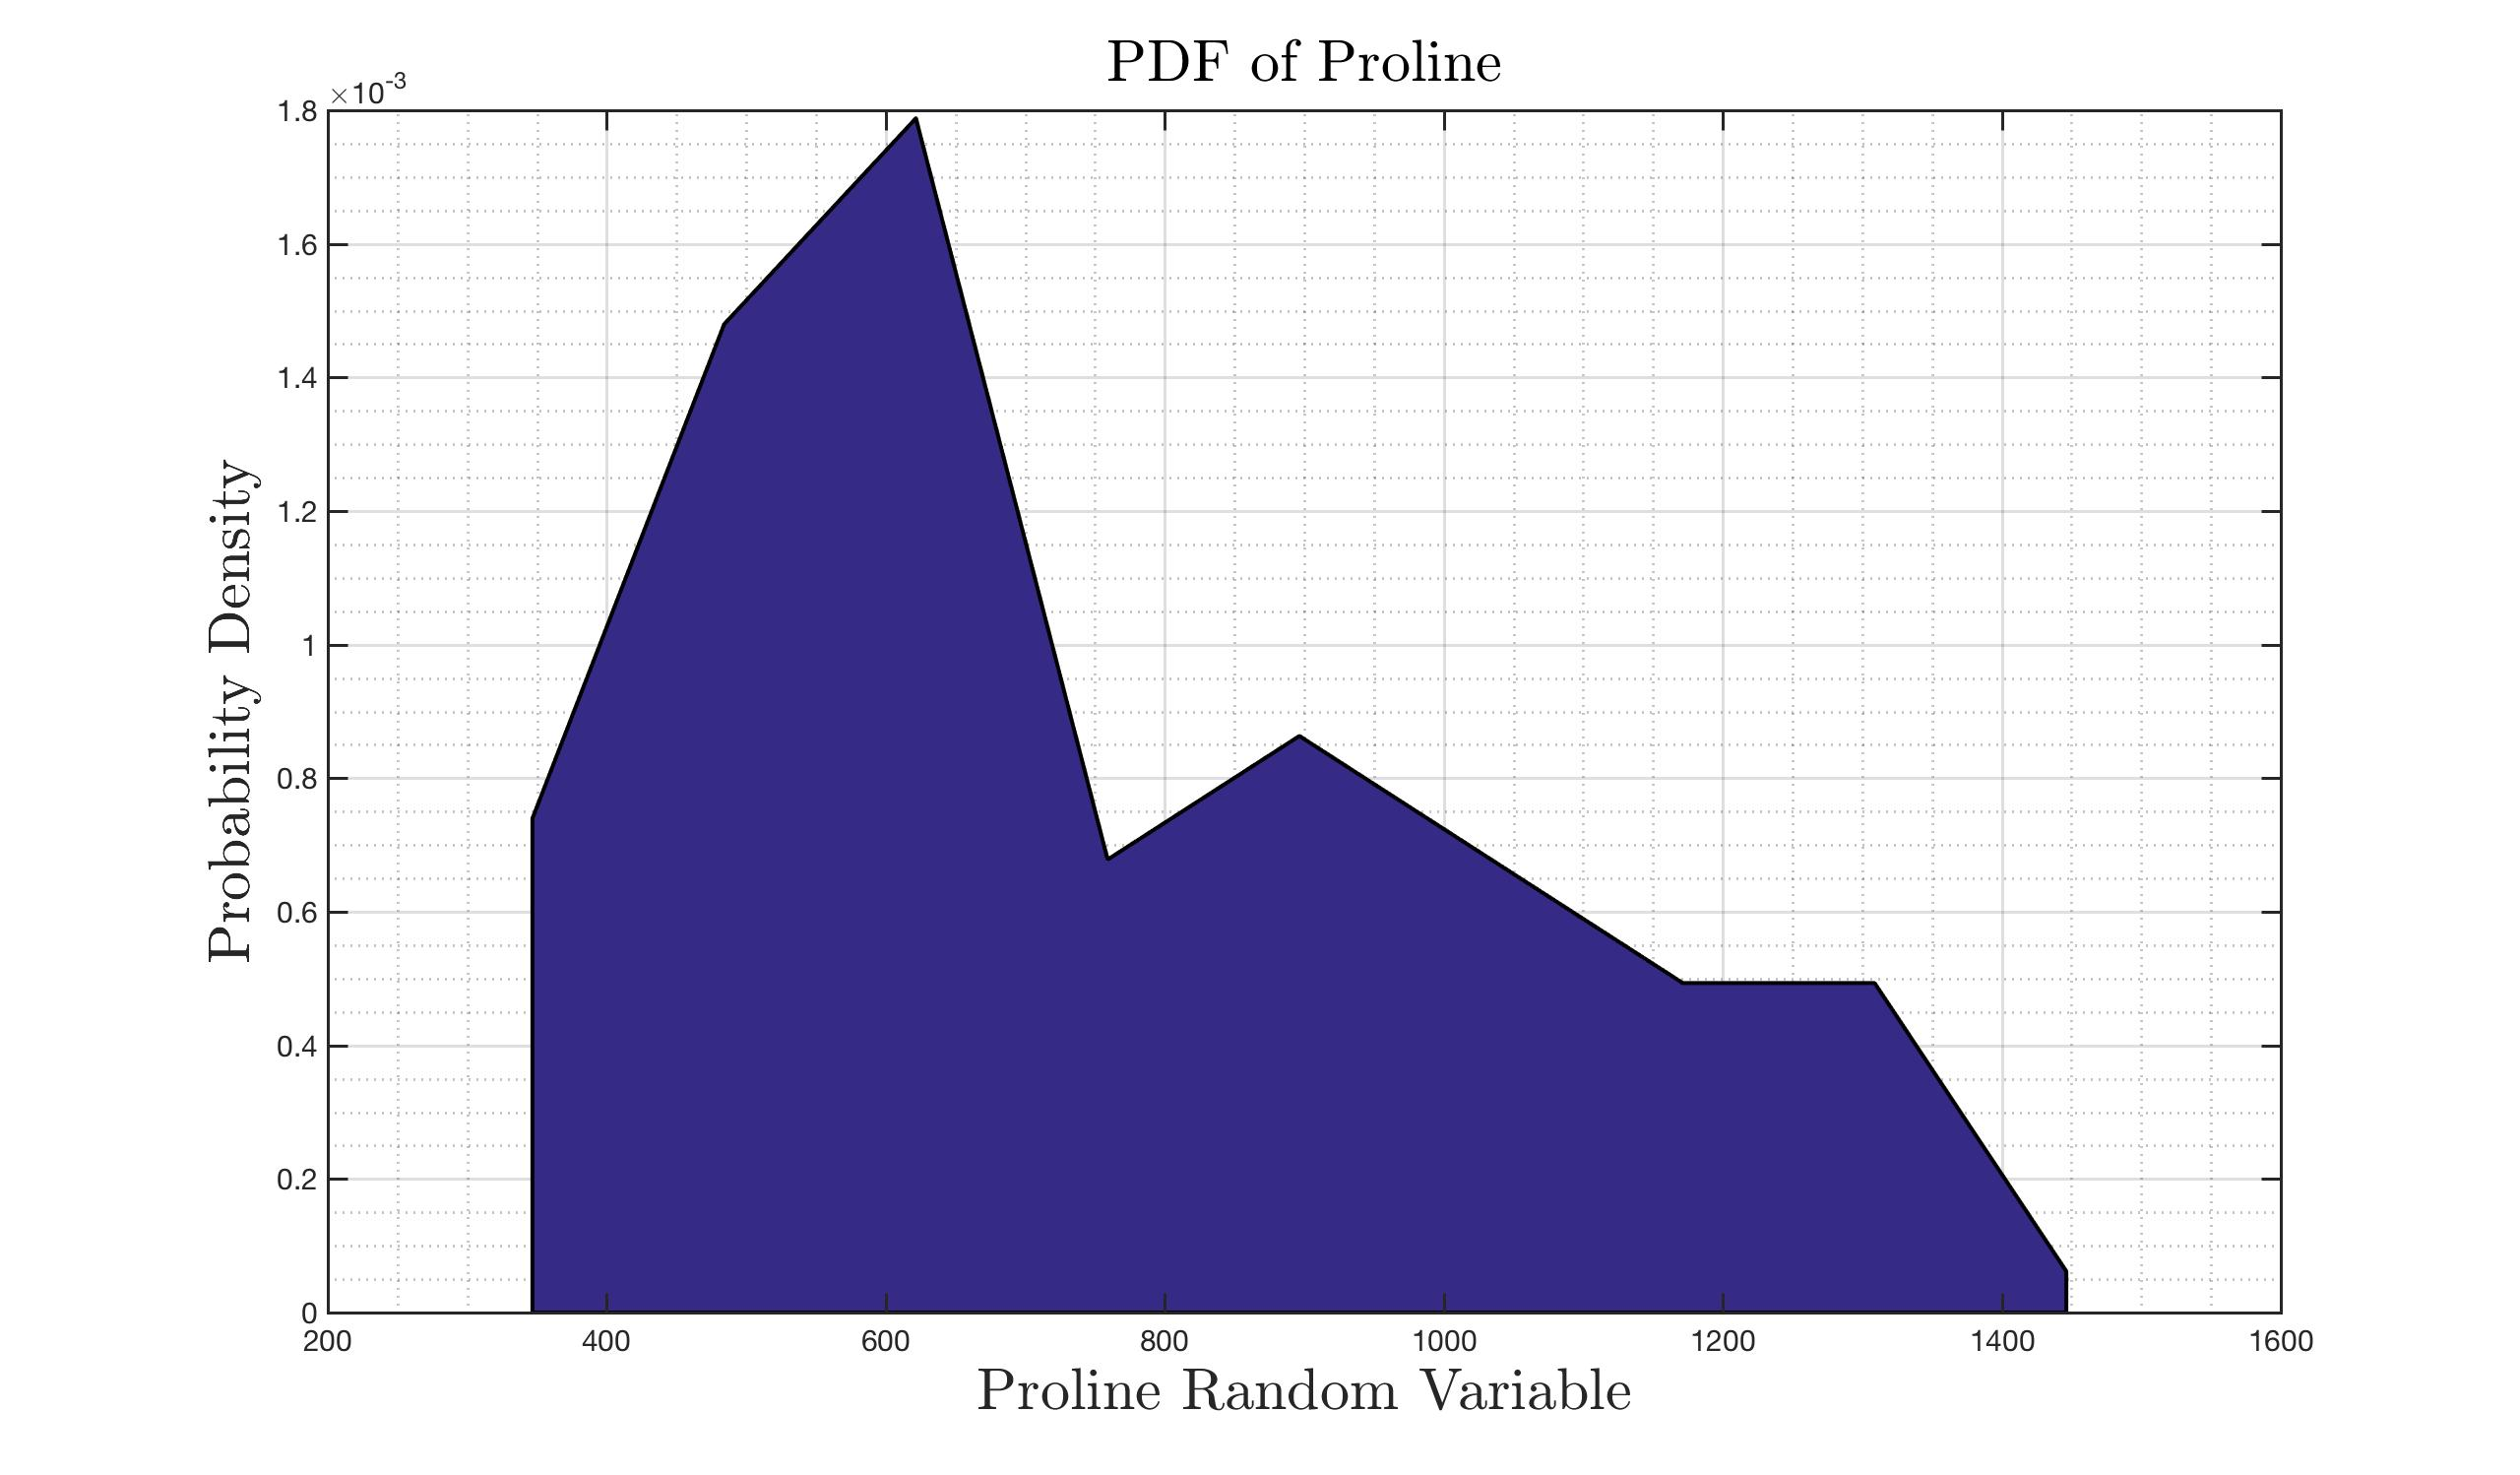
\includegraphics[width=0.4\textwidth]{../results/Q1_ProlineDist}
\caption{Distribution of Proline from all Classes \label{fig:DistProline}}
\end{figure}

\begin{table}[H]
\caption{Sample Means and Standard Dev. for all Training Data \label{tab:statAll}}
\small
\begin{center}
\begin{tabular}{|c| c c c c|}
\hline
\bf Stat/RV & Alcohol & Ash & Hue & Proline \\ [0.5ex]
\hline
\bf Mean & 12.7 & 2.38 & 0.95 & 737 \\ [0.5ex]
\hline
\bf Std. & 0.72 & 0.29 & 0.24 & 287 \\ [0.5ex]
\hline
\end{tabular}
\end{center}
\end{table}

\vspace{-5mm}

Looking at the covariance matrix of the raw training data we can see that proline covary with all other features quite strongly. This is however due to the fact that proline's distribution has a naturally high variance, thus corrupting the readings. The highest covariance for two different features excluding proline is that of magnesium (feature 5) and colour intensity (feature 10). However, these two features have second and third highest variance distributions. We have to therefore look at the covariance matrix of the normalised feature vectors.

Highest positive covariance is observed for features 6 and 7 (total phenols and flavonoids), whereas the most negative covariance is found for features 2 and 7 (malic acid and flavonoids). The plot of the above cases is shown in Figure \ref{fig:covAll}. This tells us that there is possibly some correlation between the features, e.g. increasing the phenols count increases the number of flavonoids in wine. This does in fact hold in real world, as flavonoids are a subset of natural phenols.

\begin{figure}[H]
\centering
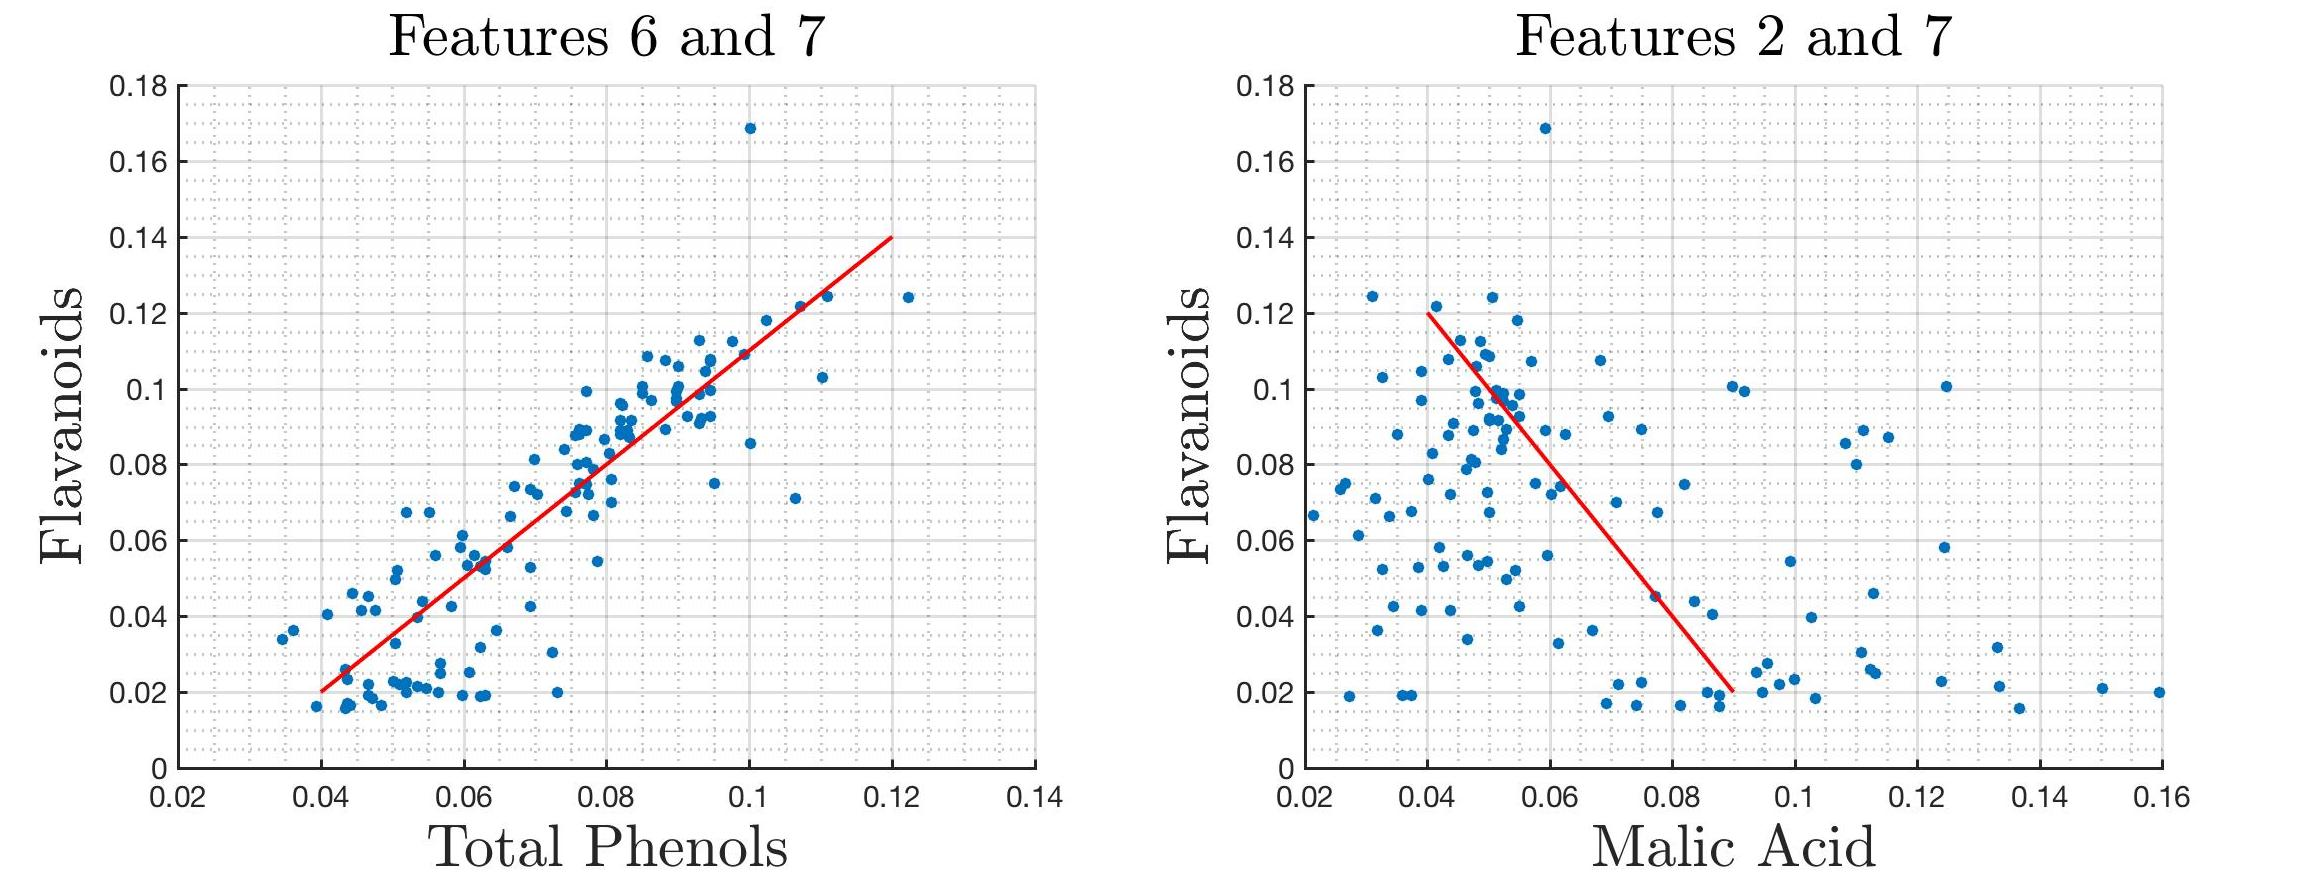
\includegraphics[width=0.5\textwidth]{../results/Q1_covAll}
\caption{Covariance of Features 6 \& 7 and 2 \& 7 Visualised \label{fig:covAll}}
\end{figure}

\vspace{-5mm}

\subsubsection{Individual Classes} \label{sec:CovCla}

\indent \indent As mentioned earlier, the PDF seen in Figure \ref{fig:DistProline} is a summation of three other PDFs for classes 1, 2 and 3. This is shown in Figure \ref{fig:DistProline_Idv}. We can see that in fact, each individual proline random variable can be estimated with a Gaussian distribution. Given that the random variables can be thought of as independent, their sum is also normally distributed.

\begin{figure}[H]
\centering
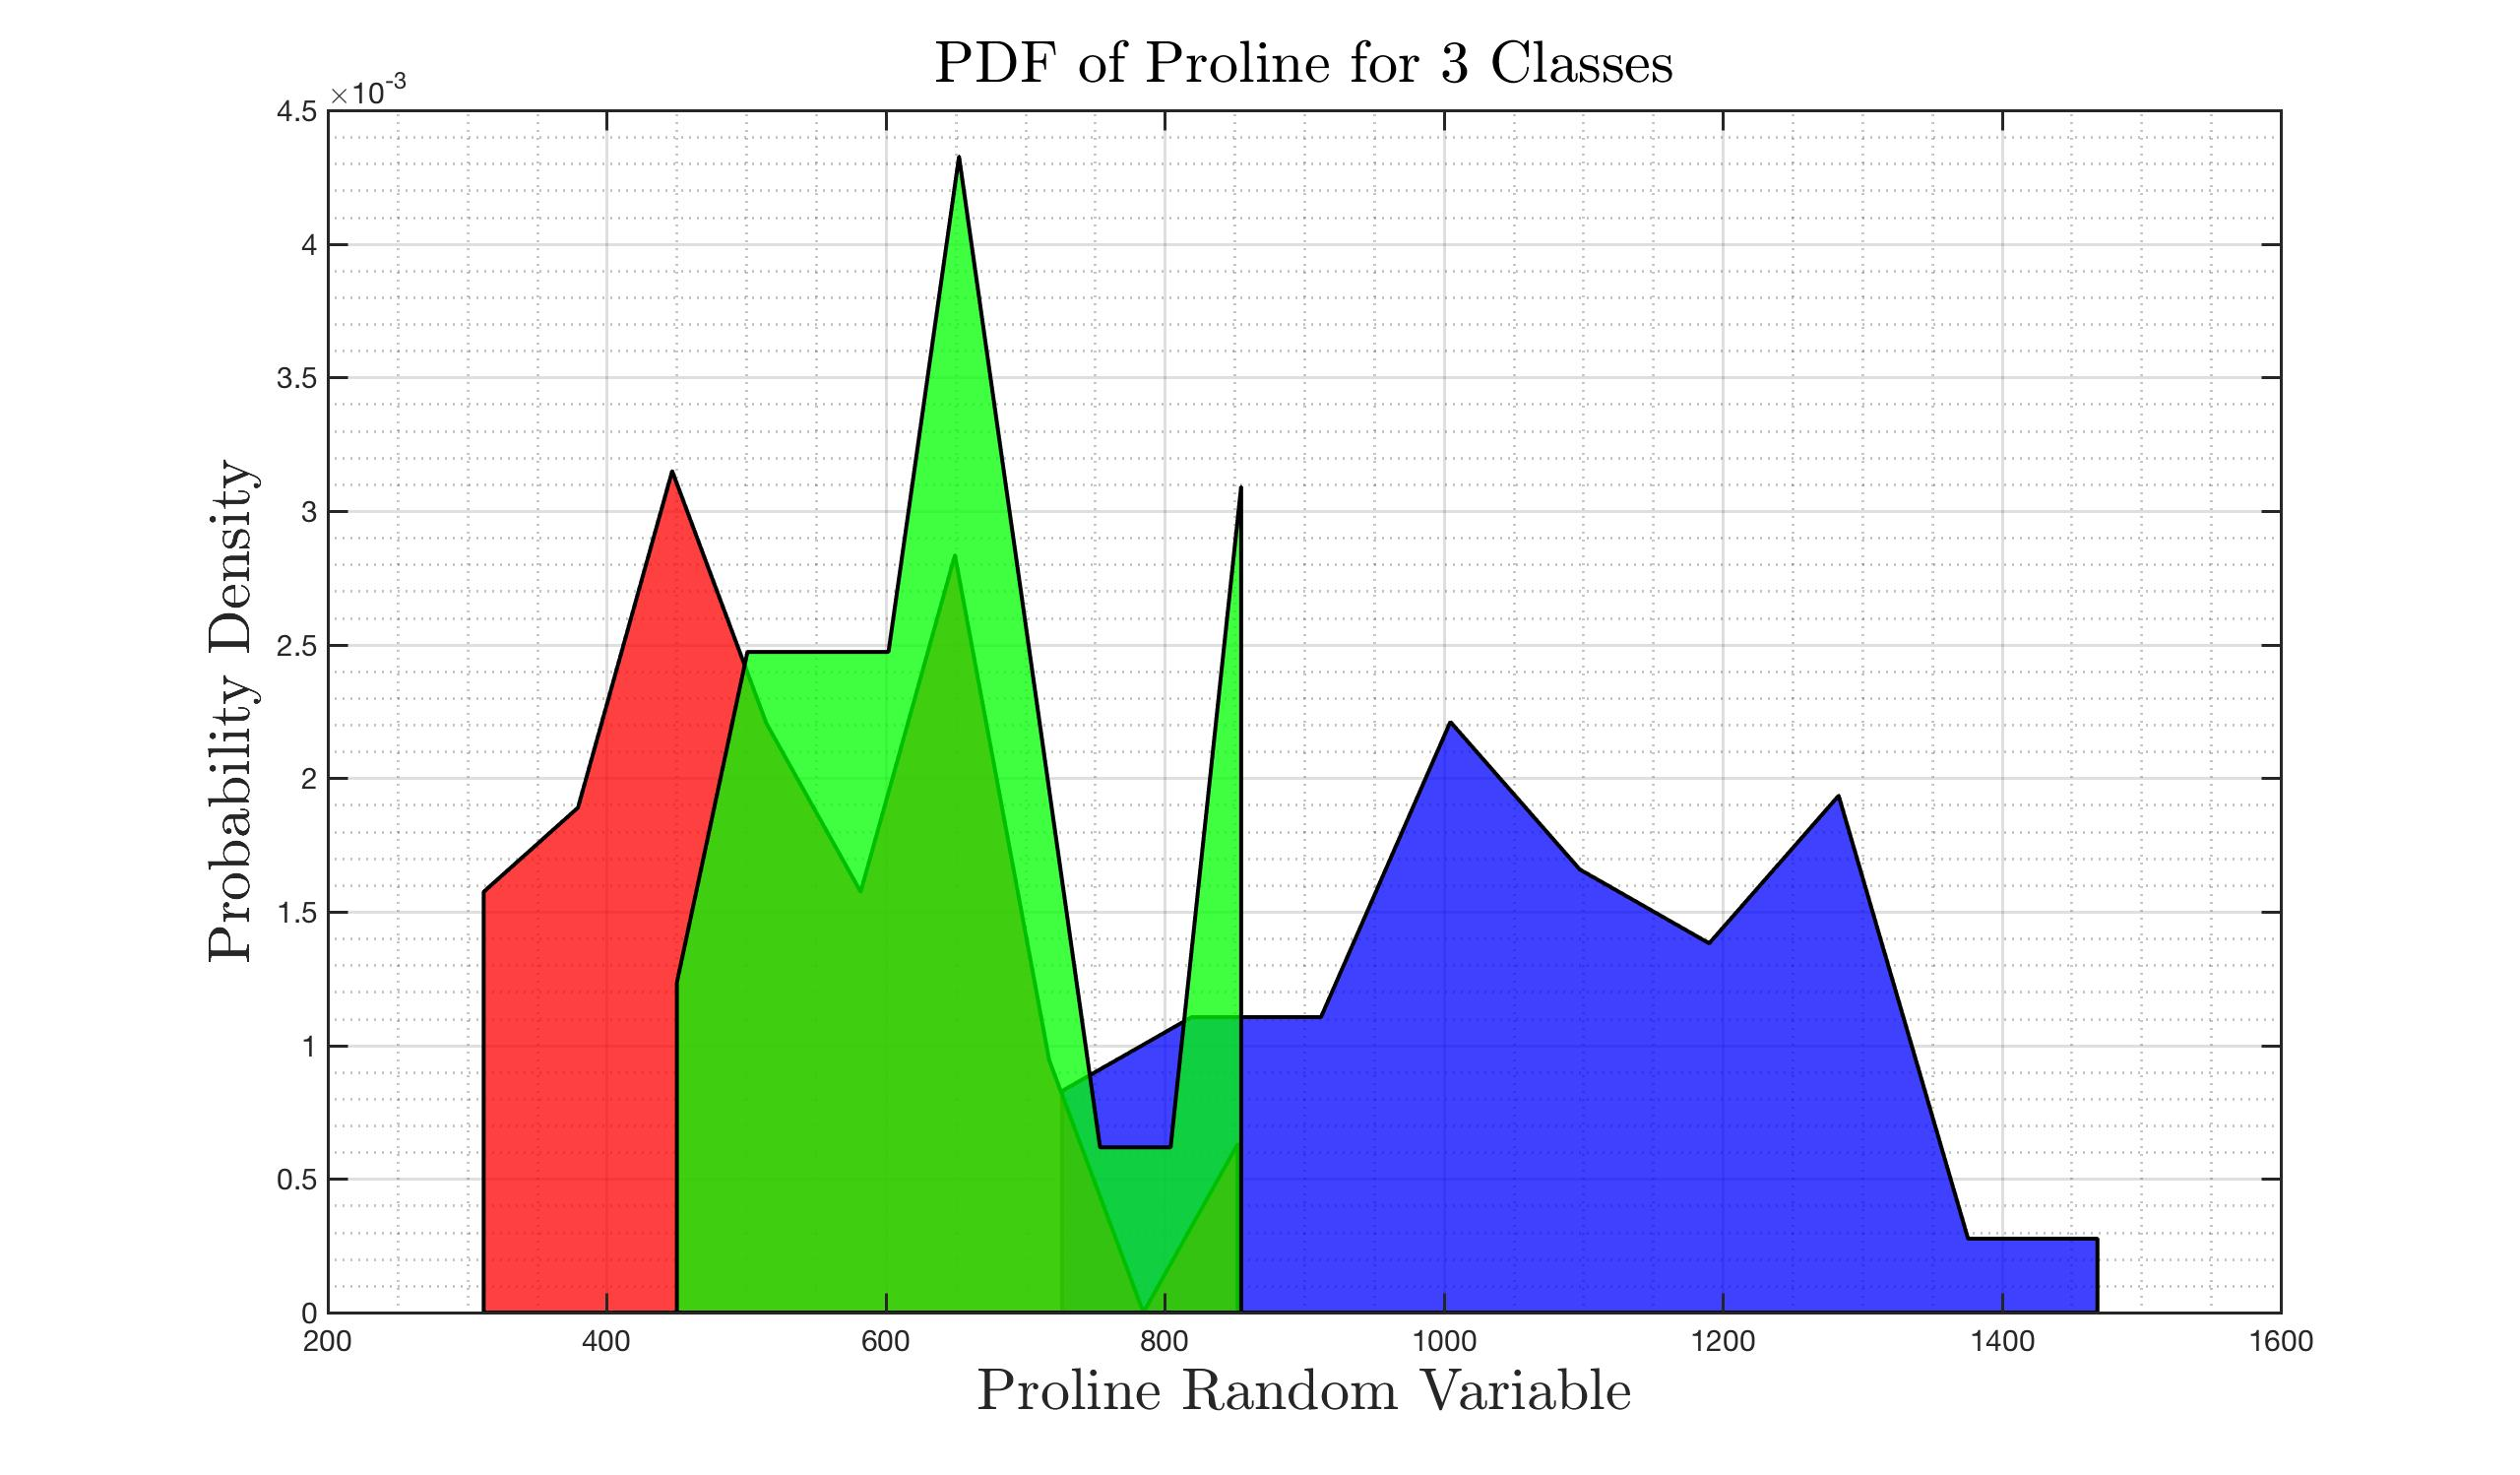
\includegraphics[width=0.4\textwidth]{../results/Q1_ProlineDist_Idv}
\caption{PDF of Proline for Class 1 (blue), 2 (red) and 3 (green) Visualised \label{fig:DistProline_Idv}}
\end{figure}

The above figure shows that each feature in every class can have a very different distribution to other classes and to the overall sum. This is the basis for feature recognition. Given that the features vary from class to class we will be able to determine the test class. For instance in Figure \ref{fig:DistProline_Idv} class 1 clearly stands out. Hence if we test a wine whose proline exceeds 900, it will most definitely belong to class 1. Let us then see how the means and standard deviations of the features in Table \ref{tab:statAll} change when we separate the data.

\begin{table}
\caption{Sample Means and Standard Dev. for each Class \label{tab:statCla}}
\small
\begin{center}
\begin{tabular}{|c| c c c c|}
\hline
\bf Stat/RV & Alcohol & Ash & Hue & Proline \\ [0.5ex]
\hline
\bf Mean 1 & 13.5 & 2.50 & 1.10 & 1070 \\ [0.5ex]
\hline
\bf Mean 2 & 12.0 & 2.27 & 1.07 & 522 \\ [0.5ex]
\hline
\bf Mean 3 & 12.9 & 2.41 & 0.67 & 647 \\ [0.5ex]
\hline
\bf Std. 1 & 0.31 & 0.26 & 0.12 & 195 \\ [0.5ex]
\hline
\bf Std. 2 & 0.32 & 0.34 & 0.21 & 145 \\ [0.5ex]
\hline
\bf Std. 3 & 0.35 & 0.18 & 0.10 & 121 \\ [0.5ex]
\hline
\end{tabular}
\end{center}
\vspace{-5mm}
\end{table}

Table \ref{tab:statCla} tells us for instance, that wine from class 1 has a higher alcohol contents than the other two classes. Wine from class 3 however is of different colour, meaning it could be a class of white or red wines. Finally, looking at proline concentration, we can see again, that class 1 stands out. A research paper \cite{wine} shows that Savignon Blanc and Grillo wines tend to have a much higher proline content than other wines, meaning this can be class of those wines.

 
After dividing the data into classes and calculating their respective covariance matrices we see that those features, which used to have a relatively large covariance, are not necessarily correlated anymore. In Figure \ref{fig:covIdv}, it can be seen that features 2 and 7 for class 3 are completely unrelated.

\begin{figure}[H]
\centering
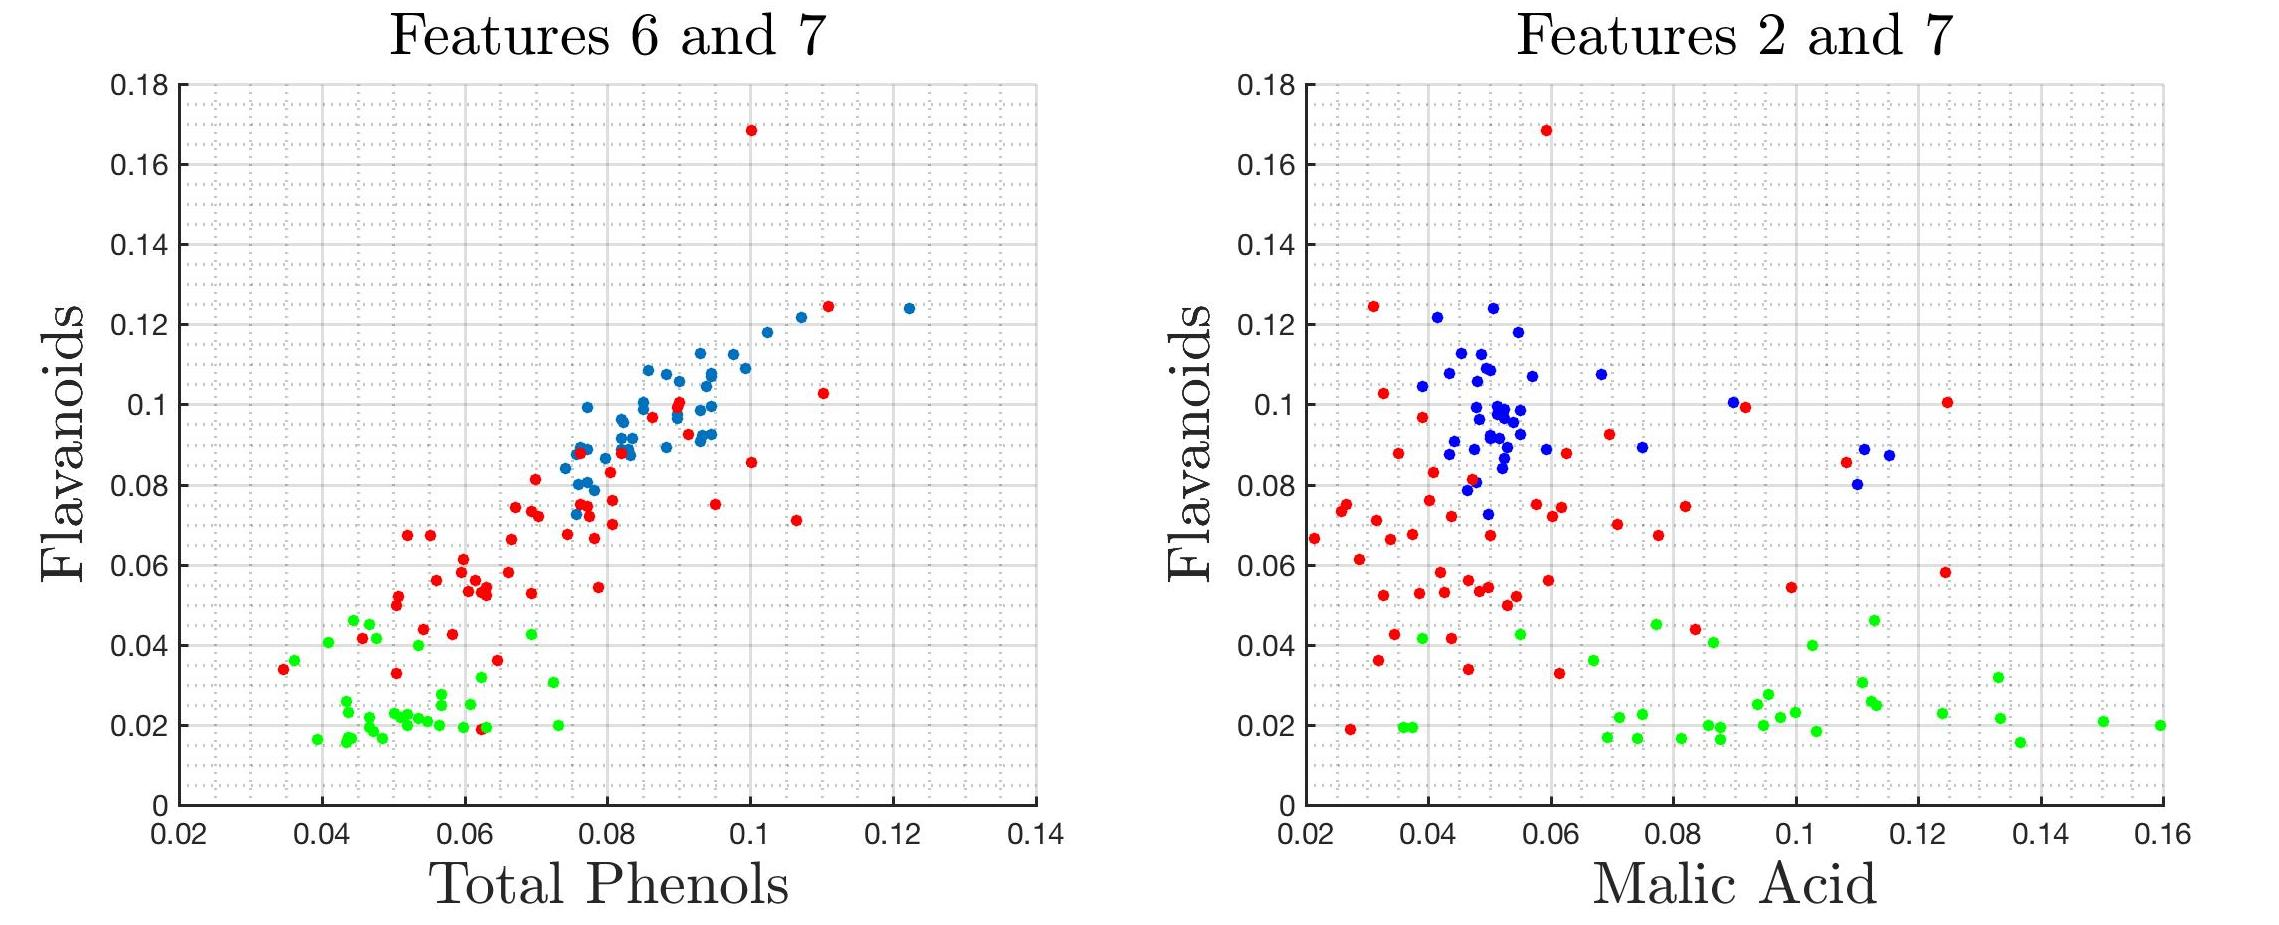
\includegraphics[width=0.5\textwidth]{../results/Q1_covIdv}
\caption{Covariance of Features 6 \& 7 and 2 \& 7  for Class 1 (blue), 2 (red) and 3 (green) Visualised \label{fig:covIdv}}
\end{figure}

\subsection{L1, L2 , Chi-Squared, Histogram Intersection, Correlation Metrics}

In order to assign class to a test wine, we need to employ some similarity measure. The simplest belong to Minkowski's Form - L1 and L2. They measure the Manhattan and Euclidean distances respectively. A more complex is to measure the chi-squared distance, which corrects the L2 metric by taking into account the absolute positions of the points in space. Hence if points have relatively large coordinates, the "hit" is allowed to be further away. Similarly, if a point of consideration has relatively small coordinates, then the match must be more precise in order to be classified as a hit. For instance an L1 metric of points $(100,0)$, $(60,0)$ and $(50,0)$, $(10,0)$ would yield 40 for both. However chi-squared distance is 5.05 and 13.7 respectively, meaning even though the two sets of points are equally spaced, the first pair is more likely to be a hit.

In the table below we have summarised the results of the above metric and also histogram intersection and correlation measure. Each metric was used for raw and normalised data.

\begin{table}[H]
\caption{Miss Rates for Various Metrics and Data Form \label{tab:MissMetric}}
\small
\begin{center}
\begin{tabular}{|c| c c c c c|}
\hline
\bf Metric & L1 & L2 & Chi-Sq. &  Hist. & Corr. \\ [0.5ex]
\hline
\bf Miss Raw & 15\% &20\%  & 10\% & 17.5\% & 20\% \\ [0.5ex]
\hline
\bf Miss Norm & 10\% & 12.5\% & 5\% & 25\% & 10\% \\ [0.5ex]
\hline
\end{tabular}
\end{center}
\end{table}

\vspace{-5mm}

The tests employed feature vectors of length 13 each as histograms, with the exception of histogram intersection. In this particular case we have used all of the training data and converted it into 3 histograms - one for each class. Then by transforming each test wine into a histogram with identical bin positions we performed the histogram intersection. We have then varied the number of bins and plotted the resulting accuracy curve. This is shown in Figure \ref{fig:hist}.

\begin{figure}[H]
\centering
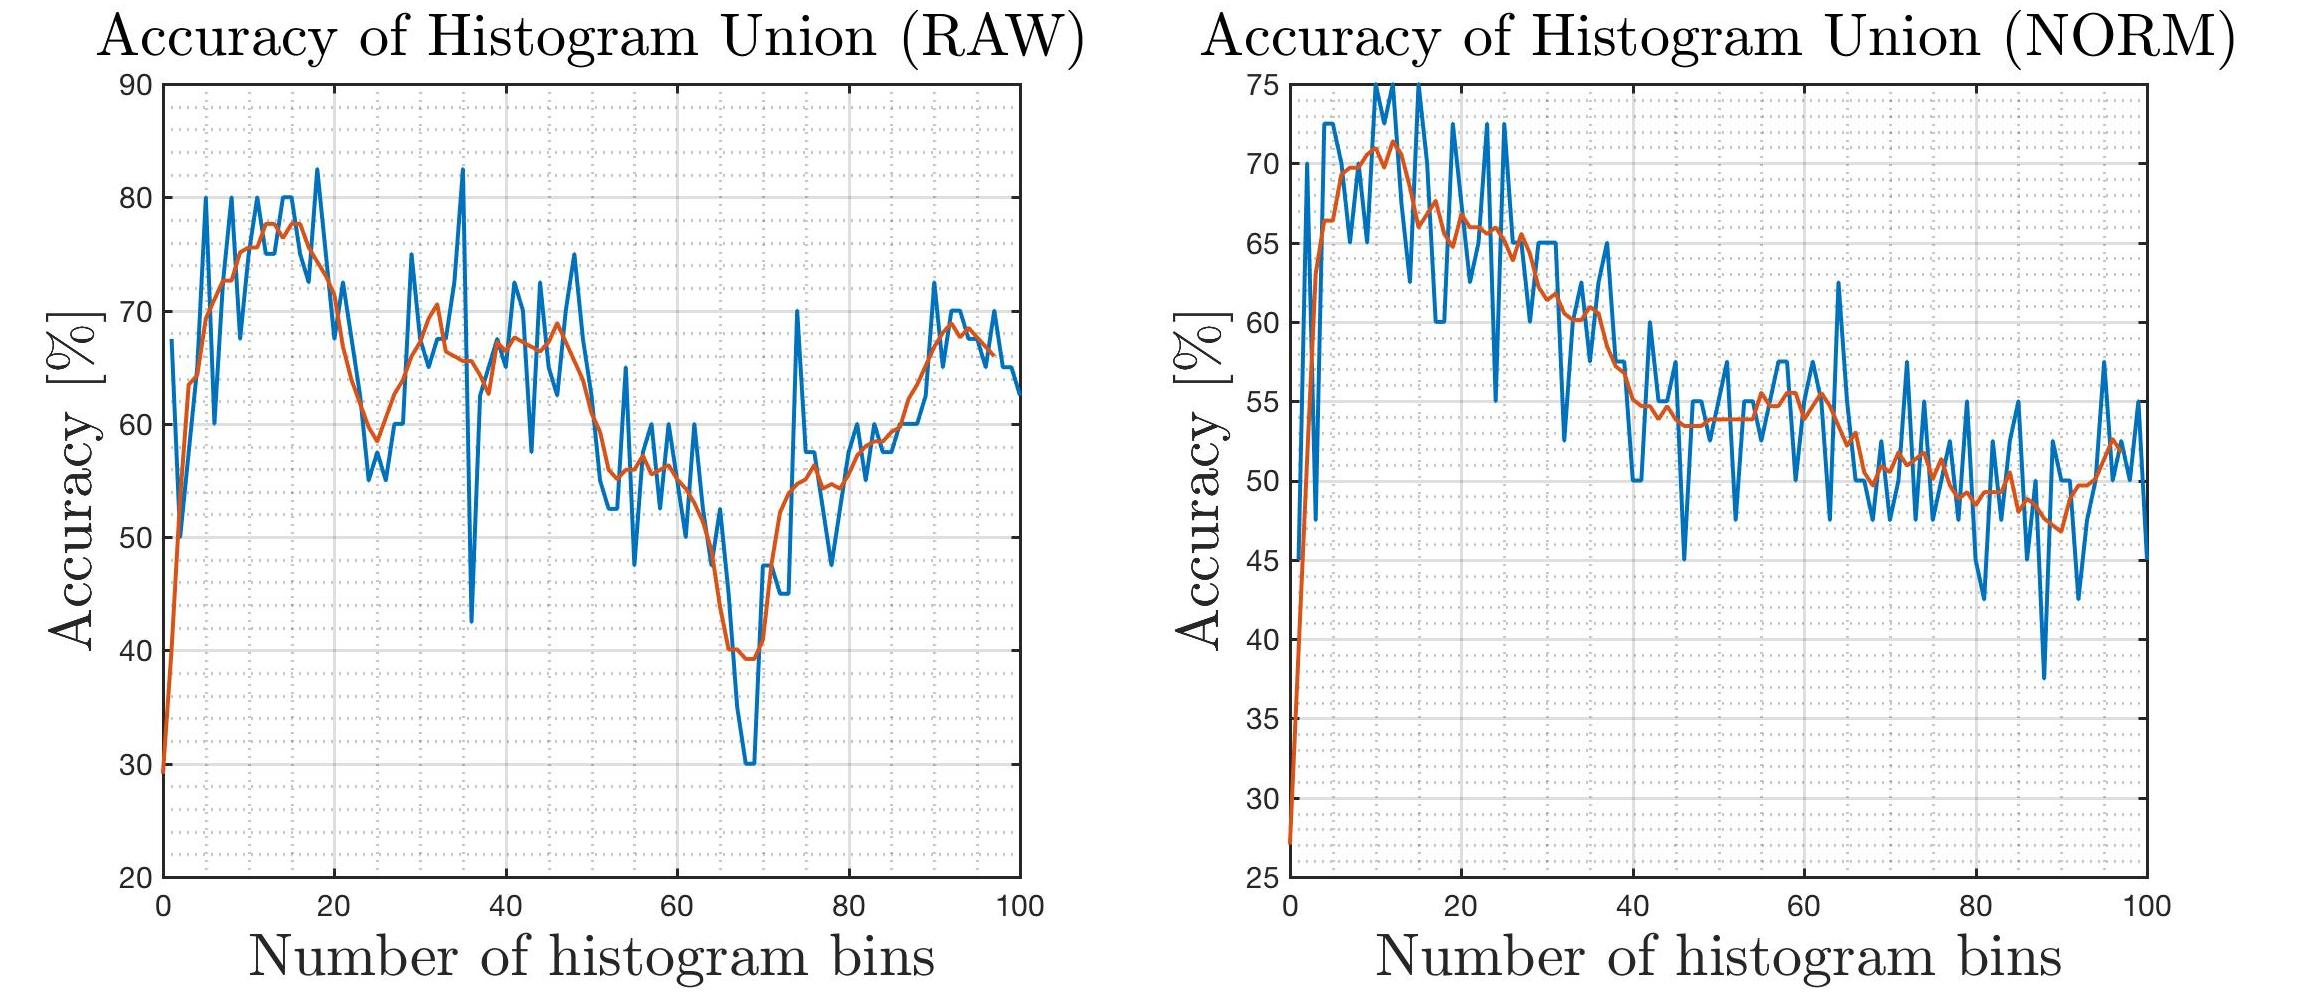
\includegraphics[width=0.5\textwidth]{../results/Q1D_Hist}
\caption{Plots of Hit Rate against Number of Bins for Raw and Normalised Data
\label{fig:hist}}
\end{figure}

Following from Table \ref{tab:MissMetric} it can be deduced that Chi-Squared metric produces best results for both sets of data - raw and normalised. It is however surprising that L1 has produced results more accurate than L2 in either case. It is said \cite{L1L2} that L2 theoretically is superior over L1 as it preserves the distance energy. However, the same source reports that there are practical situations when L1 might be better, such as when there are outliers. L1 is reported to be more robust when class occupies the space quite sparsely. In this experiment we have employed the Nearest Neighbour method. Hence the class spread is unimportant. Thus the superiority of L1 over L2 possibly comes to this particular set of training and testing data.
\subsection{Mahalanobis Distance Metric}

\section{K-means Clustering}

\section{Neural Network}

\section{Conclusion}

\begin{thebibliography}{9}
\bibitem{wine} 
C. S. Ough
\textit{Proline contents of grapes and wines}. 
Department of Viticulture and Enology, University of California, Davis, USA
\url{http://www.vitis-vea.de/admin/volltext/e054492.pdf}

\bibitem{L1L2} 
George Bebis
\textit{Advances in Visual Computing, Second International Symposium}.
ISVC 2006 Lake Tahoe, NV, USA, November 6-8, 2006. Proceedings, Part II 

\end{thebibliography}

\end{document}
